% GNUPLOT: LaTeX picture with Postscript
\begingroup
  \makeatletter
  \providecommand\color[2][]{%
    \GenericError{(gnuplot) \space\space\space\@spaces}{%
      Package color not loaded in conjunction with
      terminal option `colourtext'%
    }{See the gnuplot documentation for explanation.%
    }{Either use 'blacktext' in gnuplot or load the package
      color.sty in LaTeX.}%
    \renewcommand\color[2][]{}%
  }%
  \providecommand\includegraphics[2][]{%
    \GenericError{(gnuplot) \space\space\space\@spaces}{%
      Package graphicx or graphics not loaded%
    }{See the gnuplot documentation for explanation.%
    }{The gnuplot epslatex terminal needs graphicx.sty or graphics.sty.}%
    \renewcommand\includegraphics[2][]{}%
  }%
  \providecommand\rotatebox[2]{#2}%
  \@ifundefined{ifGPcolor}{%
    \newif\ifGPcolor
    \GPcolortrue
  }{}%
  \@ifundefined{ifGPblacktext}{%
    \newif\ifGPblacktext
    \GPblacktextfalse
  }{}%
  % define a \g@addto@macro without @ in the name:
  \let\gplgaddtomacro\g@addto@macro
  % define empty templates for all commands taking text:
  \gdef\gplbacktext{}%
  \gdef\gplfronttext{}%
  \makeatother
  \ifGPblacktext
    % no textcolor at all
    \def\colorrgb#1{}%
    \def\colorgray#1{}%
  \else
    % gray or color?
    \ifGPcolor
      \def\colorrgb#1{\color[rgb]{#1}}%
      \def\colorgray#1{\color[gray]{#1}}%
      \expandafter\def\csname LTw\endcsname{\color{white}}%
      \expandafter\def\csname LTb\endcsname{\color{black}}%
      \expandafter\def\csname LTa\endcsname{\color{black}}%
      \expandafter\def\csname LT0\endcsname{\color[rgb]{1,0,0}}%
      \expandafter\def\csname LT1\endcsname{\color[rgb]{0,1,0}}%
      \expandafter\def\csname LT2\endcsname{\color[rgb]{0,0,1}}%
      \expandafter\def\csname LT3\endcsname{\color[rgb]{1,0,1}}%
      \expandafter\def\csname LT4\endcsname{\color[rgb]{0,1,1}}%
      \expandafter\def\csname LT5\endcsname{\color[rgb]{1,1,0}}%
      \expandafter\def\csname LT6\endcsname{\color[rgb]{0,0,0}}%
      \expandafter\def\csname LT7\endcsname{\color[rgb]{1,0.3,0}}%
      \expandafter\def\csname LT8\endcsname{\color[rgb]{0.5,0.5,0.5}}%
    \else
      % gray
      \def\colorrgb#1{\color{black}}%
      \def\colorgray#1{\color[gray]{#1}}%
      \expandafter\def\csname LTw\endcsname{\color{white}}%
      \expandafter\def\csname LTb\endcsname{\color{black}}%
      \expandafter\def\csname LTa\endcsname{\color{black}}%
      \expandafter\def\csname LT0\endcsname{\color{black}}%
      \expandafter\def\csname LT1\endcsname{\color{black}}%
      \expandafter\def\csname LT2\endcsname{\color{black}}%
      \expandafter\def\csname LT3\endcsname{\color{black}}%
      \expandafter\def\csname LT4\endcsname{\color{black}}%
      \expandafter\def\csname LT5\endcsname{\color{black}}%
      \expandafter\def\csname LT6\endcsname{\color{black}}%
      \expandafter\def\csname LT7\endcsname{\color{black}}%
      \expandafter\def\csname LT8\endcsname{\color{black}}%
    \fi
  \fi
    \setlength{\unitlength}{0.0500bp}%
    \ifx\gptboxheight\undefined%
      \newlength{\gptboxheight}%
      \newlength{\gptboxwidth}%
      \newsavebox{\gptboxtext}%
    \fi%
    \setlength{\fboxrule}{0.5pt}%
    \setlength{\fboxsep}{1pt}%
\begin{picture}(7760.00,2820.00)%
    \gplgaddtomacro\gplbacktext{%
      \csname LTb\endcsname%%
      \put(212,341){\makebox(0,0){\strut{}$0$}}%
      \csname LTb\endcsname%%
      \put(636,341){\makebox(0,0){\strut{}$10$}}%
      \csname LTb\endcsname%%
      \put(1060,341){\makebox(0,0){\strut{}$20$}}%
      \csname LTb\endcsname%%
      \put(1483,341){\makebox(0,0){\strut{}$30$}}%
      \csname LTb\endcsname%%
      \put(1907,341){\makebox(0,0){\strut{}$40$}}%
      \csname LTb\endcsname%%
      \put(2331,341){\makebox(0,0){\strut{}$50$}}%
    }%
    \gplgaddtomacro\gplfronttext{%
      \csname LTb\endcsname%%
      \put(1271,109){\makebox(0,0){\strut{}$\phi$ (°)}}%
      \csname LTb\endcsname%%
      \put(1271,2587){\makebox(0,0){\strut{}\ZIFCH3}}%
      \csname LTb\endcsname%%
      \put(1759,2214){\makebox(0,0)[r]{\strut{}\scriptsize 0 \ce{N2}}}%
      \csname LTb\endcsname%%
      \put(1759,2059){\makebox(0,0)[r]{\strut{}\scriptsize 10 \ce{N2}}}%
      \csname LTb\endcsname%%
      \put(1759,1904){\makebox(0,0)[r]{\strut{}\scriptsize 25 \ce{N2}}}%
      \csname LTb\endcsname%%
      \put(1759,1749){\makebox(0,0)[r]{\strut{}\scriptsize 40 \ce{N2}}}%
      \csname LTb\endcsname%%
      \put(1759,1594){\makebox(0,0)[r]{\strut{}\scriptsize 50 \ce{N2}}}%
    }%
    \gplgaddtomacro\gplbacktext{%
      \csname LTb\endcsname%%
      \put(2628,341){\makebox(0,0){\strut{}$0$}}%
      \csname LTb\endcsname%%
      \put(3086,341){\makebox(0,0){\strut{}$10$}}%
      \csname LTb\endcsname%%
      \put(3544,341){\makebox(0,0){\strut{}$20$}}%
      \csname LTb\endcsname%%
      \put(4001,341){\makebox(0,0){\strut{}$30$}}%
      \csname LTb\endcsname%%
      \put(4459,341){\makebox(0,0){\strut{}$40$}}%
      \csname LTb\endcsname%%
      \put(4917,341){\makebox(0,0){\strut{}$50$}}%
    }%
    \gplgaddtomacro\gplfronttext{%
      \csname LTb\endcsname%%
      \put(3772,109){\makebox(0,0){\strut{}$\phi$ (°)}}%
      \csname LTb\endcsname%%
      \put(3772,2587){\makebox(0,0){\strut{}\ZIFCl}}%
      \csname LTb\endcsname%%
      \put(4345,2214){\makebox(0,0)[r]{\strut{}\scriptsize 0 \ce{N2}}}%
      \csname LTb\endcsname%%
      \put(4345,2059){\makebox(0,0)[r]{\strut{}\scriptsize 10 \ce{N2}}}%
      \csname LTb\endcsname%%
      \put(4345,1904){\makebox(0,0)[r]{\strut{}\scriptsize 25 \ce{N2}}}%
      \csname LTb\endcsname%%
      \put(4345,1749){\makebox(0,0)[r]{\strut{}\scriptsize 40 \ce{N2}}}%
      \csname LTb\endcsname%%
      \put(4345,1594){\makebox(0,0)[r]{\strut{}\scriptsize 50 \ce{N2}}}%
    }%
    \gplgaddtomacro\gplbacktext{%
      \csname LTb\endcsname%%
      \put(5215,341){\makebox(0,0){\strut{}$0$}}%
      \csname LTb\endcsname%%
      \put(5673,341){\makebox(0,0){\strut{}$10$}}%
      \csname LTb\endcsname%%
      \put(6131,341){\makebox(0,0){\strut{}$20$}}%
      \csname LTb\endcsname%%
      \put(6588,341){\makebox(0,0){\strut{}$30$}}%
      \csname LTb\endcsname%%
      \put(7046,341){\makebox(0,0){\strut{}$40$}}%
      \csname LTb\endcsname%%
      \put(7504,341){\makebox(0,0){\strut{}$50$}}%
    }%
    \gplgaddtomacro\gplfronttext{%
      \csname LTb\endcsname%%
      \put(6359,109){\makebox(0,0){\strut{}$\phi$ (°)}}%
      \csname LTb\endcsname%%
      \put(6359,2587){\makebox(0,0){\strut{}\ZIFBr}}%
      \csname LTb\endcsname%%
      \put(6932,2214){\makebox(0,0)[r]{\strut{}\scriptsize 0 \ce{N2}}}%
      \csname LTb\endcsname%%
      \put(6932,2059){\makebox(0,0)[r]{\strut{}\scriptsize 8 \ce{N2}}}%
      \csname LTb\endcsname%%
      \put(6932,1904){\makebox(0,0)[r]{\strut{}\scriptsize 20 \ce{N2}}}%
      \csname LTb\endcsname%%
      \put(6932,1749){\makebox(0,0)[r]{\strut{}\scriptsize 40 \ce{N2}}}%
      \csname LTb\endcsname%%
      \put(6932,1594){\makebox(0,0)[r]{\strut{}\scriptsize 50 \ce{N2}}}%
    }%
    \gplbacktext
    \put(0,0){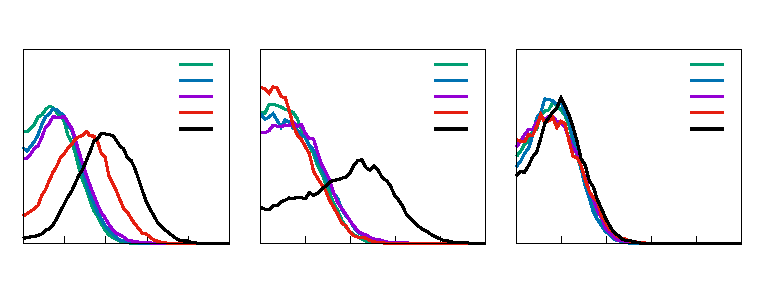
\includegraphics{zif8x-dihedrals}}%
    \gplfronttext
  \end{picture}%
\endgroup
